\documentclass[compress]{beamer}
\usetheme{hitszbeamer}
\usepackage{booktabs}
\usepackage{bm}

\begin{document}

\graphicspath{{figures/}}

\title[基于神经网络和树搜索的五子棋AI]{基于神经网络和树搜索的五子棋AI\\[2mm] 立项答辩}
\author[王梓尧]{答辩人:修泽\\[2mm] 组员:王梓尧 \hspace{2pt} 修泽}
\institute[哈尔滨工业大学]{\small  哈尔滨工业大学}
\date{\small \vskip -10pt 2023年2月4日}

\begin{frame}
  \maketitle
\end{frame}

\section*{目录}
\frame{
  \frametitle{\secname}
  \tableofcontents[hideallsubsections]
}

\section{立项背景}

\begin{frame}{立项背景}
  \begin{itemize}
    \item 2016年,AlphaGo在五番棋中击败韩国棋手李世石
    \item 2017年,AlphaGo在五番棋中 3:0 击败中国棋手,当时的等级分世界第一名柯洁        
  \end{itemize}
  \begin{figure}[htbp]
    \centering
	\begin{minipage}[t]{0.4\textwidth}
	  \centering
      
\includegraphics[width=0.9\linewidth]{alphago.jpg}
      \caption{AlphaGo}
    \end{minipage}
    \begin{minipage}[t]{0.4\textwidth}
	  \centering
      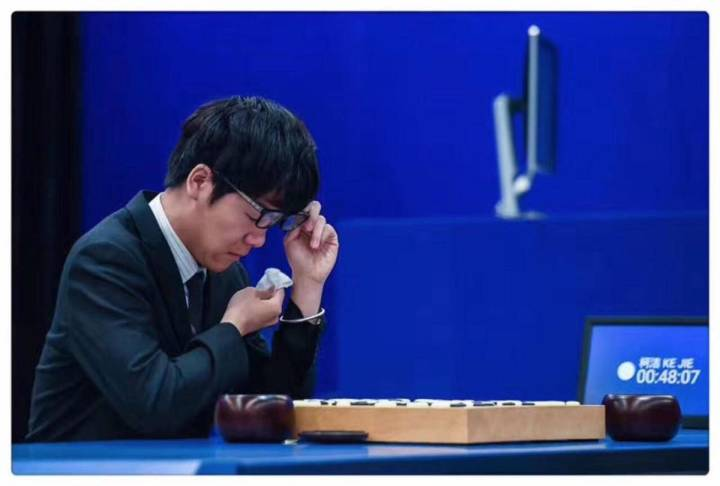
\includegraphics[width=0.9\linewidth]{Kejie.jpg}
      \caption{柯洁落败}
    \end{minipage}
  \end{figure}
\end{frame}


\begin{frame}{立项背景}
  \begin{itemize}
    \item 自主训练,不需要数据集
          \pause
    \item 方案成熟,预期的成功率和强度较高
  \end{itemize}
\end{frame}

\section{实施方案}

\subsection{技术栈}

\begin{frame}{技术栈}
  \begin{figure}[htbp]
    \centering
    \begin{minipage}[t]{0.4\textwidth}
      \centering
      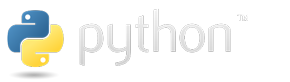
\includegraphics[width=3cm]{python-logo.png}
    \end{minipage}
    \\[5mm]
    \begin{minipage}[t]{0.4\textwidth}
      \centering
      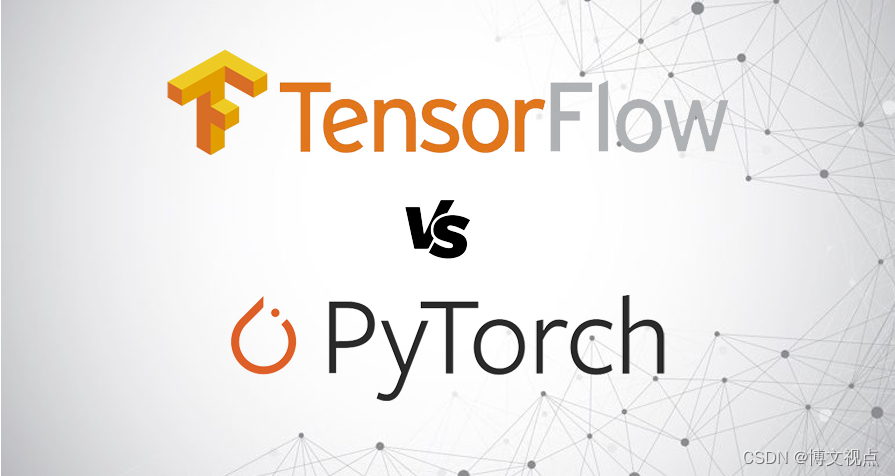
\includegraphics[width=3cm]{d7f4837cf8284e08838d13669f8eb738.png}
    \end{minipage}
  \end{figure}
\end{frame}

\subsection{基本原理}

\subsubsection{模型训练}

\begin{frame}{模型训练}
  \begin{block}{应用算法}
    \begin{itemize}
      \setlength{\itemsep}{6pt}
      \item 蒙特卡罗树搜索 (MCTS)
      \item 残差网络 (ResNet)
    \end{itemize}
  \end{block}
  \begin{figure}[htbp]
    \centering
    \begin{minipage}[t]{0.4\textwidth}
      \centering
      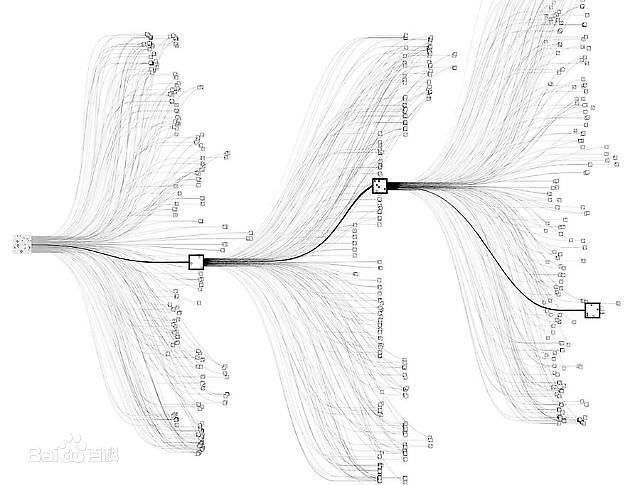
\includegraphics[width=0.9\linewidth]{mc.jpg}
      \caption{MCTS}
    \end{minipage}
    \begin{minipage}[t]{0.4\textwidth}
      \centering
      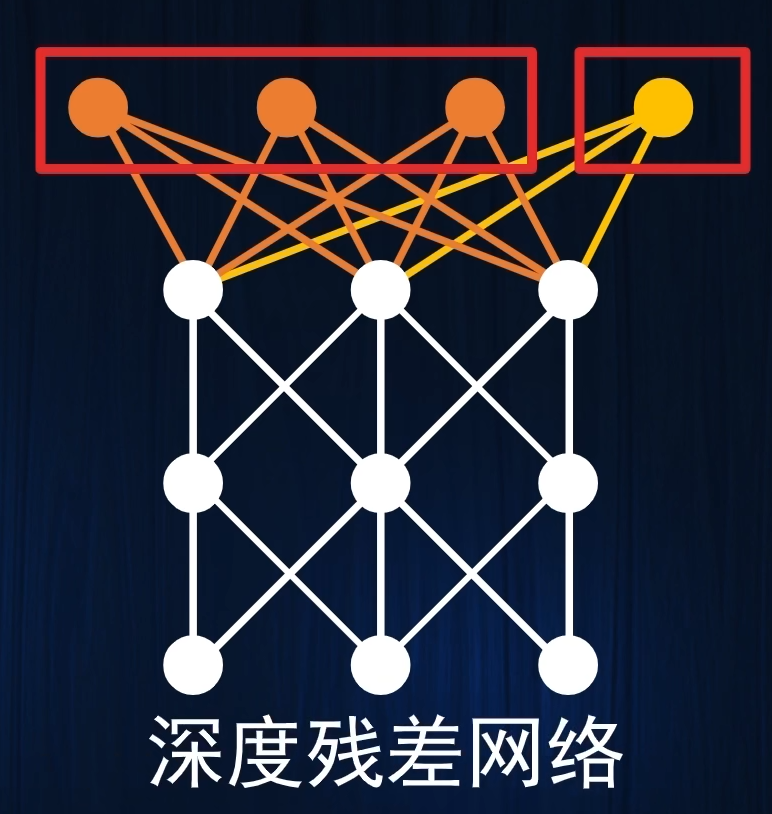
\includegraphics[width=0.9\linewidth]{resnet.png}
      \caption{ResNet}
    \end{minipage}
  \end{figure}
\end{frame}

\begin{frame}{模型训练}
  \begin{figure}
    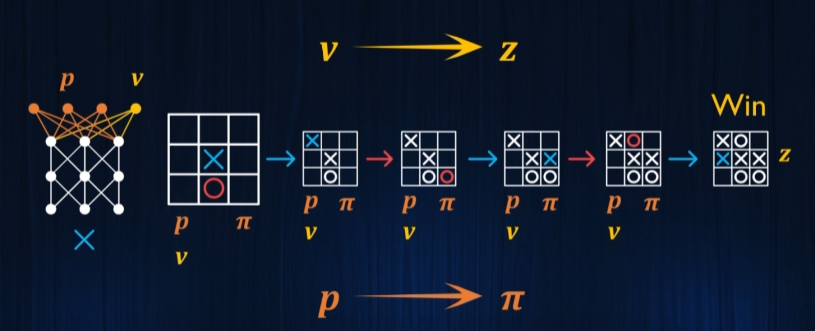
\includegraphics[width=0.9\linewidth]{mt.png}
    \caption{ResNet拟合目标}
  \end{figure}
\end{frame}

\begin{frame}{模型训练}
  \begin{figure}
    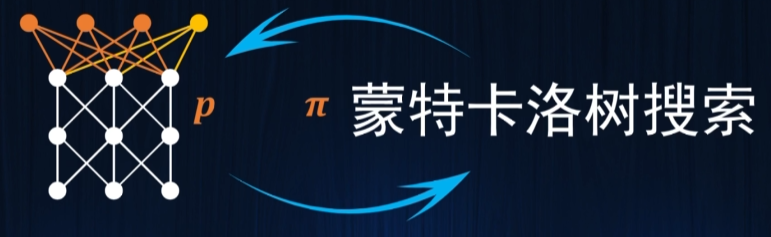
\includegraphics[width=0.9\linewidth]{mt2.png}
    \caption{训练过程}
  \end{figure}
\end{frame}

\section{预期目标}

\begin{frame}{预期目标}
  \begin{block}{中期}
    \begin{itemize}
      \setlength{\itemsep}{6pt}
      \item 完成后端系统开发
      \item 及时总结反思
    \end{itemize}
  \end{block}
\end{frame}

\begin{frame}{预期目标}
  \begin{block}{结题}
    \begin{itemize}
      \setlength{\itemsep}{6pt}
      \item 完成五子棋AI
            \begin{itemize}
              \setlength{\itemsep}{6pt}
              \item 较快的运行速度
              \item 较强的对弈水平
              
            \end{itemize}
      \item 完成五子棋AI
            \begin{itemize}
            \setlength{\itemsep}{6pt}
            \item 支持人机对弈
            \item 界面简洁友好
            \item 支持难度调整
            \end{itemize}
            
    \end{itemize}
  \end{block}
\end{frame}

\section{Q\&A}

\begin{frame}{\secname~ }
  \begin{center}
    \huge{That's all. Thank you!}\\
    \vspace{1cm}
    \huge{Q\&A}
  \end{center}
\end{frame}

\end{document}
